\documentclass[11pt]{article}

\topmargin -.5in
\evensidemargin 0in
\oddsidemargin 0in
\textheight 9in
\textwidth 6.5in
\usepackage{url}
\usepackage{graphicx}
\usepackage{amsmath,amssymb,amsfonts}
\newtheorem{theorem}{Theorem}
\usepackage{float}
\usepackage{mathtools}


\begin{document}

\section*{Design and Implementation of Air Pollution Monitoring System}

The progress in technology has made it easy for researchers to explore more in different areas. One such development is in the area of sensor technology which completely changed the outlook of different application level problems. In this chapter, I share my hands-on experience in the development, design, integration, and operation of the air pollution system using commodity sensor. Earlier, the approach for understanding air pollution used complex and stationary equipment which collects data and used these data for analyzing, but things have changed after the low cost, easy to use, portable sensors came in markets \cite{Snyder2013}. 

\section*{Design Goals}

There are many factors which need to be considered for the development of a simple yet reliable system. In this section, we have mentioned the factors which should be considered for an effective air pollution monitoring system.

\begin {enumerate}

\item{Sensor Identification}

The very first task is to figure out which all sensors need to be included for the completion of the system. There are sensors available in the market for the measurement of almost all types of gases in the atmosphere. It should be very clear that which all gases need to be measured and this definitely changes from region to region as in certain places the concentration of a particular gas is more. Having said that, there will be a certain set of gases which must be included for measurement regardless of the region.

\item{Communication Module}

As the system is completely based on wireless sensors the selection of data transmission is another crucial factor. The communication between the server and the sensors should be taken into consideration.
The collected data from the sensors should be transferred over a database or to the sever. For that the type of communication module can be either Wi-Fi or bluetooth module.
 
\item {Reliability}

The success of the system depends upon how much accurate the data is. The value which we obtain from the sensor should make sense to the audience. There will be a lot of noise coming with the  collection of data, the sensor should have the ability to remove the noise data or it should allow the programmer to make changes or apply certain algorithm so that the data sets will be refined.


\item {Easy Integration}

The integration of sensors with the processor is one important factor that needs to be kept in mind. Some sensors can be easily integrated with any processor but others needs driver codes to be written in order to work with the processor.

\item {Printed Circuit Board}

The final system should be build on a printed circuit board as it is more dependable. Circuit build on basic breadboard might even come out as it is not permanently fixed and this will cause frequent breakdown. Its always easy to work on breadboard but that will be useful only for the initial set up. The system should be transformed to PCB.


\item {Maintenance}

In case of any sensor damage it should be easily replaceable which means the complete system should be a plug and play type model. On building up such a  model like that will help in debugging the problems caused by sensors if any. It should also be considered that the sensors selected for the system should be easily available in market so that it can be replaced if needed.

\item {Easy Replication}
The idea behind creating such a system is that it can be replicated by anyone without even knowing the dept knowledge. The system should be designed in such a way that it should use the most available sensors and processors in the market. The programming part of the sensors to processor will be easy if the selection of processor is simple. This could definitely bring down a lot of work done at the hardware level.


\item {Low Cost}

Within the available sensors in the market one could find sensors ranging from a very low price to costliest of all. There was a budget set for the the complete system and finding the right sensors with the affordable cost is one crucial factor.

\end{enumerate}


\section*{Targeted Pollutants}

Our surrounding is filled with various gases, these gases will become harmful if the concentration of it increases to an undesired level. On the development of a air pollution system measurement of all the gases in the atmosphere is not necessary as the collected data from all the sensor will make no sense to the public. Our main idea here is to make the general people aware about the dominant gases and the extend of health hazard caused by these gases. This can be identified through different indexes know as Air Quality Health Index(AQHI) which is a scale from one to ten developed by health and environmental professionals \cite{faq} and Air Quality index (AQI)which gives the level of air quality status in an area \cite{Asha2017}.

\par 

The development of such indexes by the scientists will give the general public more idea of the pollution. The main gases to be included for the measurement for the indexes are  $PM_{2.5}, O_3, NO_2$, and $CO$ along with temperature and humidity sensor for awareness. These gases are mainly caused due to industrialization, urbanization and motorization \cite{Saha1952}. Industrial and vehicles release greenhouse emissions which are largely responsible for air pollution \cite{ internet}. The sensors thus can be limited to five which will also make the system compact.


   \section*{Sensor Selection} 
    
    Sensor networks are new instruments useful to detect the conditions in remote places in the physical world in environmental monitoring applications such as pollution monitoring, transportation management, intrusion detection and many more \cite{Jung2011}. With the constant development in electronics industry, it is possible to collect data remotely and collected data can be transferred to the required platform at a short period of time.
    There are different sensors available in market which can measure the pollutants and display the value, but the idea here is to select the one which is of low cost and also gives the most accurate values.
    \par
    Having said that there is a variety of options available for sensors based on the way it measures the pollutants. One such category is Metal Oxide Semiconductor (MOS) gas sensor also known as semiconductor gas sensor, which is used to detect the concentration of any hazardous gases in the atmosphere by changing its resistance. The most popular series available in market for this category is MQ-XX sensors which is popular for its wide detecting scope, long life, stability, high sensitivity, fast response and also simple drive circuit \cite{Data2012}.The sensing material is made up either from Aluminum Oxide ($ Al_{2}O_{3}$) or Tungsten trioxide ($WO3$)based ceramic and has a coating of Tin Oxide $ SnO_{2} $ that acts as the sensing material for the desired gas. The sensing element is heated through Platinum wires which is connected to leads made up of Nickel-Chromium, well known conductive alloy. The gas to be detected has a specific temperature at which it gets ionized and the task of the sensor is to work at that temperature. Once the gas gets ionized it gets absorbed by the sensing material which changes the resistance and inturn changes the voltage across the sensor and can be read by the microcontroller \cite{gassensor}. The voltage value along with reference voltage and other resistor's resistance is used to find the resistance of sensor. Once the resistance of the sensor is known then by using the sensitivity curve the concentration could be found out. One such sensor used here to detect carbon monoxide is MQ-2 sensor which detects more than one gases such as LPG, Propane, and Hydrogen. The sensitivity curve for the sensor is shown for different types of gases.



    \begin{figure}
      \begin{center}
      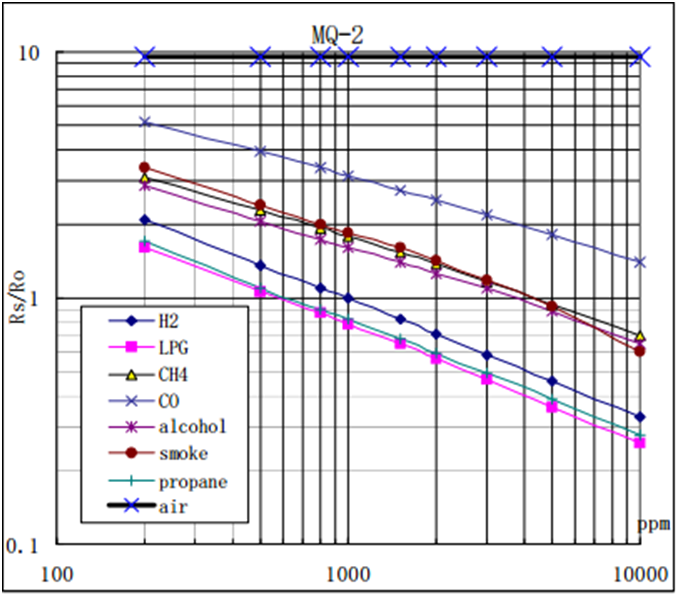
\includegraphics[scale=0.40]{images/figure1.png}
      \end{center}
      \caption{Sensitivity characteristics curve \cite{Data2012}}
      \label{mesh}
  
      where $R_{o}$ is the sensor resistance in clean air and $R_{s}$ is the sensor resistance when exposed to gas.
    \end{figure}

   \par
   From the curve above the voltage across the sensor is found out depending on which gas one wants to detect and there after using this voltage value the concentration of pollutant is calculated.

    Another popularly used  MOS sensor which we explored was MICS which are MEMS based whose mode of operation is similar to the above said sensor as both of them are metal oxide. Here, oxidizing gas or the pollutant gas add to the insulative oxygen species causing the resistance to increase \cite{SGXSensortech}.
     Other than MOS sensors, we also took a look at optical sensor which are spectroscopic devices which uses light scattering principle to find the concentration of pollutants. It consists of led, lens and photo diode inside the sensor. As soon as there is a change in concentration the photo diode detects which causes change in the current from the diode and this is how the pollutant concentration is detected \cite{Allen2002}. This sensor is known for its detecting capability of particulate matter of different sizes and is one of the recent development in the field of air quality monitoring. Highly responsive, reliable and long life are the main highlights of this sensor.

     \section*{System Architecture}
    
     In this section we describe the architecture for air pollution monitoring system which include a hardware side and a software side.The system is designed in such a way that it collects the data through the sensors, performs certain mathematical equation on the collected data and calculate the indexes then transfer these data to an IoT platform where it is visualized. The hardware section includes multiple sensors, processor and also on the wireless communication module for transmitting and receiving signals. Second, we will discuss the software side which includes the visualization part. The complete overview of the system is as shown in the figure and each part along with the sensor specification, implementation, design will be discussed further in the section. 


     \begin{figure}
      \begin{center}
      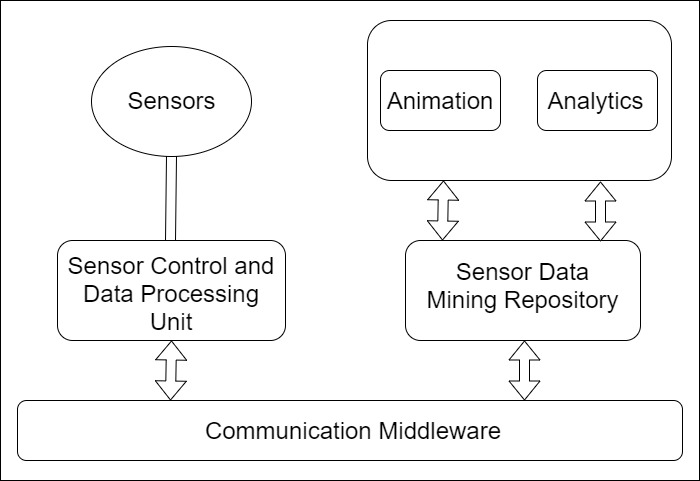
\includegraphics[scale=0.80]{images/figure2.png}
      \end{center}
      \caption{System Architecture}
      \label{mesh}
  
    \end{figure}


     \subsection*{Hardware Architecture}
\subsubsection*{Sensor Control and Data Processing Unit}
This unit is the core for the pollution monitoring as it is where all the other modules are connected including the communication middleware. This module does the following function:
\begin{enumerate}
\item It filters and processes the collected data and forward to the software.
\item Control the sensors in collecting data.
\item Provide the necessary voltage for all the hardware connected to it.
\end{enumerate}


     
     


    

    
\bibliographystyle{plain}
\bibliography{chapter3}
\end{document}
\end{document}